\documentclass[tikz,border=10pt]{standalone}
% Shared style for all Speed Demon diagrams: one palette, rounded white boxes,
% dark ink, white page (readable on GitHub light and dark).
\hyphenpenalty=10000 \exhyphenpenalty=10000 \tolerance=9999
\usepackage[T1]{fontenc}
\usepackage[scaled=0.95]{helvet}
\renewcommand{\familydefault}{\sfdefault}
\usepackage{tikz}
\usepackage{pgfplots}
\pgfplotsset{compat=1.16}
\usetikzlibrary{arrows.meta,positioning,shapes.geometric,fit,backgrounds,calc}

\definecolor{ink}{HTML}{1F2937}
\definecolor{mute}{HTML}{6B7280}
\definecolor{rule}{HTML}{9CA3AF}
\definecolor{cA}{HTML}{2563EB}   % Track A  blue
\definecolor{cB}{HTML}{D97706}   % Track B  amber
\definecolor{cC}{HTML}{059669}   % Track C  green
\definecolor{cD}{HTML}{7C3AED}   % Track D  violet
\definecolor{warn}{HTML}{DC2626} % fallback / redo path
\definecolor{wash}{HTML}{F3F4F6}

\tikzset{
  every node/.style={font=\small, text=ink},
  >={Stealth[length=2.4mm,width=1.8mm]},
  box/.style={draw=ink, fill=white, rounded corners=3pt, line width=0.7pt,
    align=center, inner sep=5pt, minimum height=12mm, text width=#1},
  box/.default=44mm,
  accent/.style={draw=#1, line width=1.2pt},
  accent/.default=cA,
  hl/.style={fill=#1!10, draw=#1, line width=1.1pt},
  dec/.style={diamond, aspect=2.6, draw=ink, fill=white, line width=0.7pt,
    align=center, inner sep=2pt, text width=#1},
  dec/.default=34mm,
  arr/.style={->, line width=0.9pt, color=ink},
  redo/.style={->, line width=0.9pt, color=warn, dash pattern=on 4pt off 3pt},
  lab/.style={font=\footnotesize, text=mute, inner sep=2pt},
  grp/.style={draw=#1, dashed, line width=0.9pt, rounded corners=6pt, inner sep=9pt,
    fill=#1!4},
  grp/.default=mute,
  grplabel/.style={font=\footnotesize\bfseries, text=#1, inner sep=2pt},
  show background rectangle,
  background rectangle/.style={fill=white, rounded corners=0pt},
}
\pgfplotsset{
  every axis/.append style={font=\small, tick label style={font=\footnotesize},
    axis line style={ink}, tick style={ink}, grid style={rule!50},
    label style={font=\small}, title style={font=\small\bfseries}},
}

% node text: \nt{title}{detail}
\newcommand{\nt}[2]{\textbf{#1}\par\vspace{1pt}{\footnotesize #2}}

\begin{document}
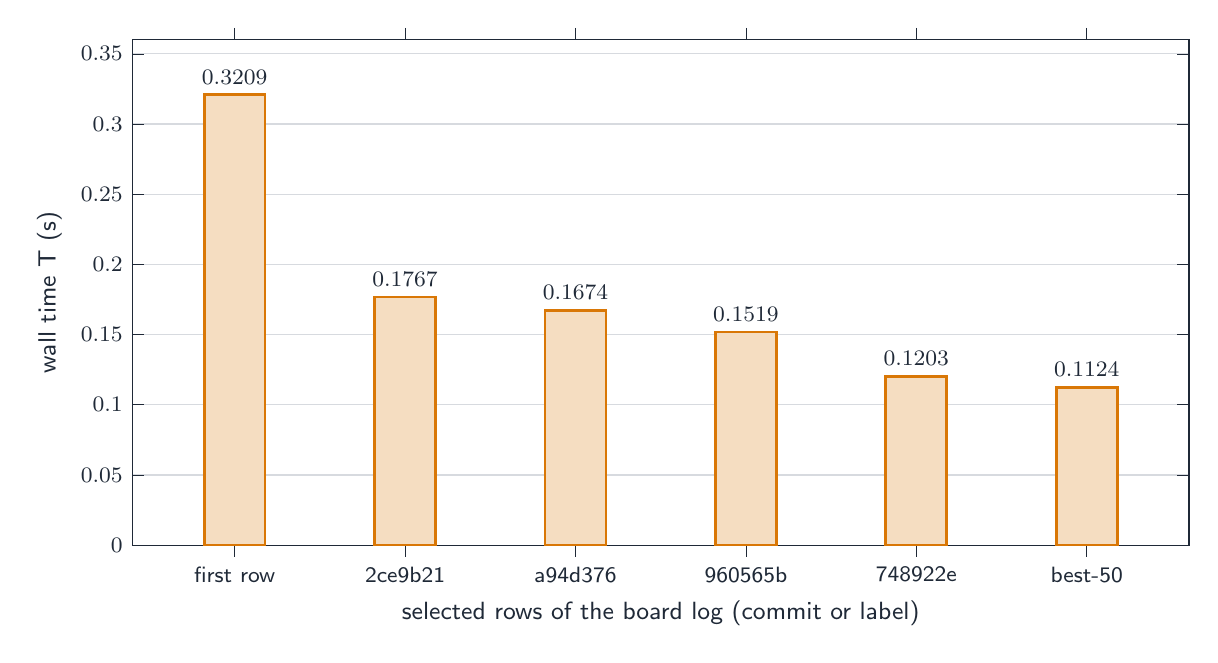
\begin{tikzpicture}
\begin{axis}[
  width=15cm, height=8cm,
  ybar, bar width=22pt,
  ymin=0, ymax=0.36, ytick distance=0.05,
  ylabel={wall time T (s)},
  symbolic x coords={first row,2ce9b21,a94d376,960565b,748922e,best-50},
  xtick=data, scaled y ticks=false, yticklabel style={/pgf/number format/fixed, /pgf/number format/precision=2},
  xlabel={selected rows of the board log (commit or label)},
  ymajorgrids, grid style={rule!40},
  enlarge x limits=0.12,
  nodes near coords, nodes near coords style={font=\footnotesize, /pgf/number format/fixed, /pgf/number format/precision=4, /pgf/number format/zerofill},
]
\addplot[fill=cB!25, draw=cB, line width=1pt] coordinates {(first row,0.3209) (2ce9b21,0.1767) (a94d376,0.1674) (960565b,0.1519) (748922e,0.1203) (best-50,0.1124)};
\end{axis}
\end{tikzpicture}
\end{document}
